\chapter{进程与进程调度}\label{cha:latex-brief-intro}

\section{实验内容}
进程切换;丰富中断处理程序,比如让时钟中断处理可以不停地发生而不是只发生一次,进程状态的保存与恢复,进程调度,解决中断重入问题。

\section{代码分析}

\subsection{核心数据结构}

\begin{table}[H]
\begin{center}
\caption{主要数据结构}
\begin{tabular}{|c|l|l|}
\hline
\multirow{2}{*}{结构体} & STACK\_FRAME       & 进程表结构体的定义 \\ \cline{2-3} 
                     & PROCESS            & 进程结构体的定义  \\ \hline
\multirow{2}{*}{宏}   & NR\_TASKS          & 最大允许进程  \\ \cline{2-3} 
                     & STACK\_SIZE\_TOTAL & 栈的大小      \\ \hline
\end{tabular}
\end{center}
\end{table}


\subsection{关键代码分析}

\begin{enumerate}
    \item 进程切换,实现从 Ring 0 到 Ring 1 的切换:\par
        当发生中断时,从内核栈切换到进程栈,指向就绪队列中下一个应该被执行的进程,同时用 TSS 保存 Ring 0 的信息,如图 7-1 所示:
        \begin{lstlisting}[language = C]
          mov  esp, [p_proc_ready]    
          lldt [esp + P_LDT_SEL]
          lea  eax, [esp + P_STACKTOP]
          mov  dword [tss + TSS3_S_SP0], eax
        \end{lstlisting}
        
        取出下一个进程所需的寄存器值,利用 \texttt{iretd} 转到 Ring 1 特权级,执行该进程,如下所示:
        \begin{lstlisting}[language = C]
          pop  gs
          pop  fs
          pop  es
          pop  ds
          popad
          add  esp, 4
          iretd
        \end{lstlisting}
    
    \item 丰富中断处理程序,让时钟中断处理可以不停发生,并在进行进程调度的时候做到进程的保存与恢复。让中断可以不停发生,设置 EOI,如下所示:
    \begin{lstlisting}[language = C]
    hwint00:
      mov  al, EOI
      out  INT_M_CTL, al
      iretd
    \end{lstlisting}
    
    为了让被中断的进程能够顺利恢复,在进程表中,我们给每一个寄存器预留了位置,以便让他们把所有的值都保存下来,这样在进程切换的时候就不会对进程产生不良影响。使用 \texttt{push} 保存原寄存器值,如下所示:
    \begin{lstlisting}[language = C]
      pushad
      push  ds
      push  es
      push  fs
      push  gs
    \end{lstlisting}
    
    使用 \texttt{pop} 恢复原寄存器值,如下所示:
    \begin{lstlisting}[language = C]
      pop  gs
      pop  fs
      pop  es
      pop  ds
      popad
    \end{lstlisting}

    
    为了保存内核栈信息,在从 Ring 0 到 Ring 1 的时候,我们使用 TSS 保存 Ring 0 的信息。在每一次重新开始前,使用 \texttt{iretd} 返回 Ring 1 之前,我们都要进行检查,以确保 \texttt{tss.esp0} 是正确的,如下所示:
    \begin{lstlisting}[language = C]
      lea  eax, [esp + P_STACKTOP]
      mov  dword [tss + TSS3_S_SP0], eax
    \end{lstlisting}
    
    \item 解决中断重入问题:
    如果中断处理完成之前就会有下一个中断产生,我们会发现中断一直在进行,不会回到我们的程序。为解决中断重入问题,我们在 \texttt{main.c} 中设置全局变量 \texttt{k\_reenter}。该全局变量初值为 -1,中断处理程序开始执行时它自加,结束时自减。在处理程序开头处,这个变量需要被检查一下,如果值不是 0,则说明在一次中断未处理完之前就又发生了一次中断,这时直接跳到最后,结束中断处理程序的执行。然后判断是否需要跳转,如果 \texttt{k\_reenter} 不为 0,则直接结束当前中断,恢复上一个进程的执行,如下所示:
    \begin{lstlisting}[language = C]
      k_reenter = -1;
    \end{lstlisting}
    
    \begin{lstlisting}[language = C]
      inc  dword [k_reenter]
      cmp  dword [k_reenter], 0
      jne  .re_enter
    \end{lstlisting}
    
    \begin{lstlisting}[language = C]
    .re_enter:
      dec  dword [k_reenter]
      pop  gs
      pop  fs
      pop  ds
      popad
      add  esp, 4
      iretd
    \end{lstlisting}
    
    \item 进程调度:
    发生时钟中断时选择进程表中的下一个进程来执行,现在我们希望设定进程的优先级。为每个进程添加一个变量 \texttt{ticks},初始值为进程的优先级。每次进程获得一个运行周期,\texttt{ticks} 减 1,减到 0 时,此进程不再获得执行机会,直到所有进程的 \texttt{ticks} 都减为 0。首先定义变量,如下所示:
    \begin{lstlisting}[language = C]
      proc_table[0].ticks = proc_table[0].priority = 150;
      proc_table[1].ticks = proc_table[1].priority = 50;
      proc_table[2].ticks = proc_table[2].priority = 30;
    \end{lstlisting}
    
    然后编写进程调度函数
    \texttt{schedule()},放在 \texttt{proc.c} 中,如下所示:
    \begin{lstlisting}[language = C]
    PUBLIC  void  schedule(){
      PROCESS* p;
      int  greatest_ticks = 0;
      while (!greatest_ticks){
        for (p = proc_table; p < proc_table + NR_TASKS; p++){
          if (p -> ticks > greatest_ticks){
            greatest_ticks = p -> ticks;
            p_proc_ready = p;
          }
          if (!greatest_ticks){
            for (p = proc_table; p < proc_table + NR_TASKS; p++){
              p ->ticks = p-> priority;
            }
          }
        }
      }
    }
    \end{lstlisting}
    
    同时修改时钟中断处理,如下所示:
    \begin{lstlisting}[language = C]
    PUBLIC  void  clock_handler(int irq){
      ticks++;
      p_proc_ready -> ticks++;
      if (k_reenter != 0){
        return;
      }
      schedule();
    }
    \end{lstlisting}
\end{enumerate}


\section{调试过程及结果分析}
由于使用的是64位系统,与参考书版本不一致,需对Makefile作一定修改:\par
CFLAGS	= -I include/ -c -fno-builtin LDFLAGS	= -s -Ttext \$(ENTRYPOINT)\par
DASMFLAGS	= -u -o \$(ENTRYPOINT) -e \$(ENTRYOFFSET)\par
改为:\par
CFLAGS	= -m32 -I include/ -c -fno-builtin -fno-stack-protector LDFLAGS	= -m elf$\_$i386 -s -Ttext \$(ENTRYPOINT)\par
DASMFLAGS	= -u -o \$(ENTRYPOINT) -e \$(ENTRYOFFSET) -m32\par
即可使用make指令直接完成编译等工作,后续调试方法与之前实验一致,进程切换实验结果如下图7-1所示:
\begin{figure}[H]
  \centering
  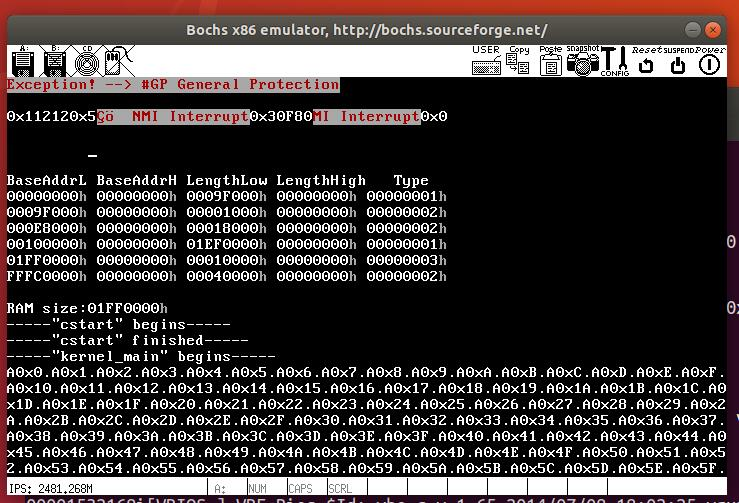
\includegraphics[width=0.8\textwidth]{figures/chapter7/7-1.jpg}
  \caption{进程切换实验结果}
  \label{fig:1}
\end{figure}

接着丰富中断处理程序,让时钟中断处理可以不停地发生而不是只发生一次,如下图7-2所示:
\begin{figure}[H]
  \centering
  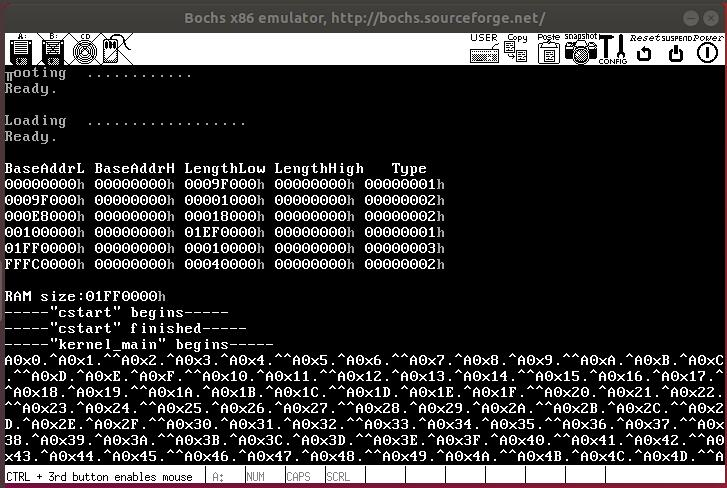
\includegraphics[width=0.8\textwidth]{figures/chapter7/7-2.jpg}
  \caption{中断不停发生实验结果}
  \label{fig:2}
\end{figure}

再实现进程状态的保存与恢复,如下图7-3所示:
\begin{figure}[H]
  \centering
  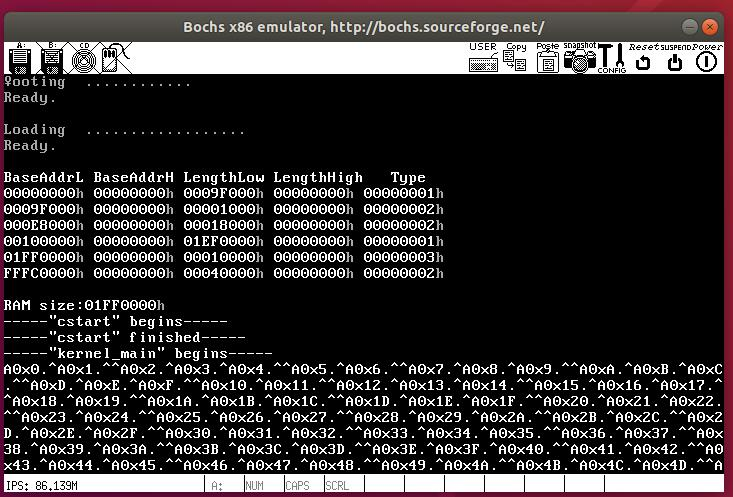
\includegraphics[width=0.8\textwidth]{figures/chapter7/7-3.jpg}
  \caption{中断不停发生实验结果}
  \label{fig:3}
\end{figure}

然后支持中断重入,如下图7-4所示:
\begin{figure}[H]
  \centering
  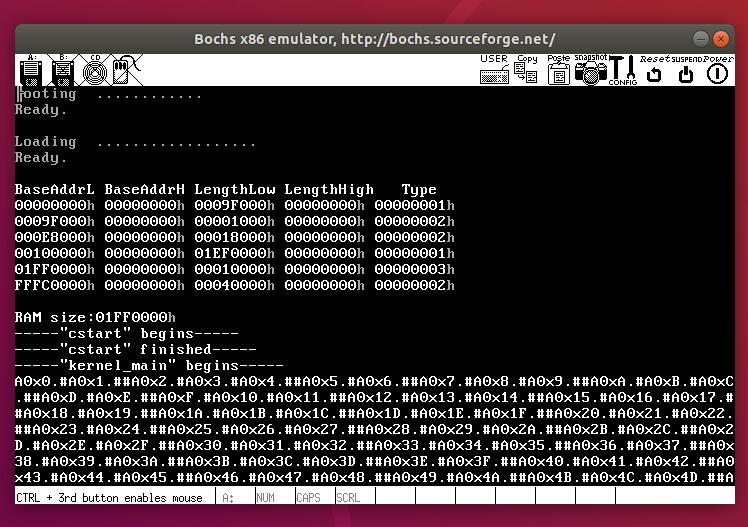
\includegraphics[width=0.8\textwidth]{figures/chapter7/7-4.jpg}
  \caption{中断重入实验结果}
  \label{fig:4}
\end{figure}

最后执行进程调度,如下图7-5所示:
\begin{figure}[H]
  \centering
  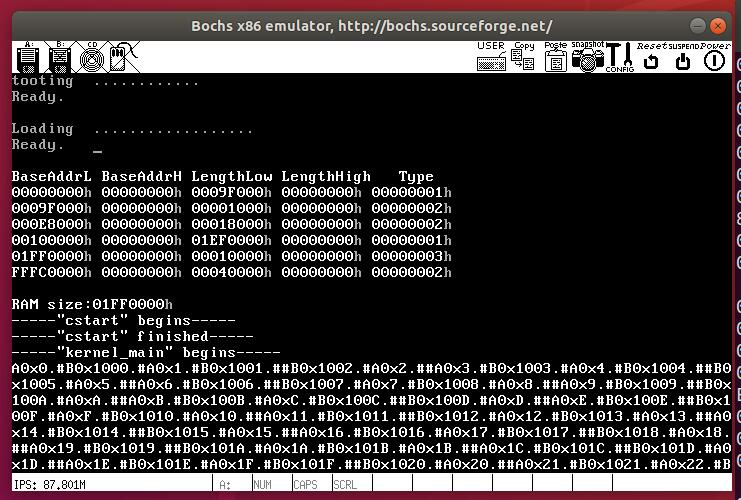
\includegraphics[width=0.8\textwidth]{figures/chapter7/7-5.jpg}
  \caption{进程调度实验结果}
  \label{fig:5}
\end{figure}

\section{实验总结}
本实验将重点放到了进程上。从进程切换,中断处理程序的丰富,再到进程切换时进程状态的保存与恢复,最后到进程调度,同时考虑并解决了中断重入问题。虽然还没办法进行输入输出,但已经可以说这个操作系统已经是一个基本完善的操作系统了。\par
本次实验使用了 Makefile 来化简我们的操作步骤以及展现不一样的内核效果。操作途中遇到了 Makefile 需要更改的问题,因为里面的内容是以 32 位虚拟机为对象来做的,而我们使用的是 64位虚拟机,将对应代码更改完后直接运行make指令,后续实验步骤和之前相同。\par
总而言之,第六个实验的任务是实现进程和进程调度。首先准备好进程体,初始化相应的描述符,准备进程表,完成特权级别的跳转,从 ring0 到 ring1。接下来要完善时钟中断处理程序,为此我们需要设置 EOI,运行可以看到 0行 0 列的字符不断变化,说明中断处理程序正在运行。然后是现场的保护和恢复,我们需要用进程表保存进程的状态,具体需要保存各寄存器的值,切内核栈和重新将 esp 切到进程表。然后是中断重入,如果中断未处理完之前又发生中断,直接结束中断处理程序的运行。实现多进程时,我们读取不同的任务地址入口、堆栈栈顶和进程名,在进程切换时重新加载 ldtr。进程切换时,为 esp 赋不同的值。我们只打开时钟中断的时候,屏蔽掉时间中断,并进行相关系统调用。在进程调度中,我们设置不同的延迟,进行了简单的优先级设置。整理的实验六的思维导图如下:
\begin{figure}[H]
  \centering
  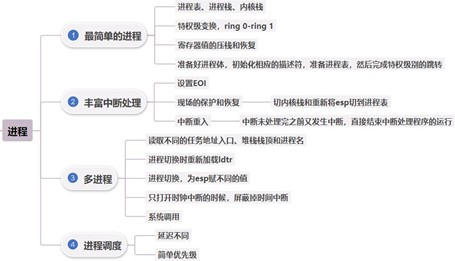
\includegraphics[width=0.8\textwidth]{figures/chapter7/7-6.jpg}
  \caption{实验六思维导图}
  \label{fig:6}
\end{figure}


